%!TEX root = ../main.tex

\newpage
\section*{Supplementary}

  {\color{red} Tables S1-S5 will be moved to GitHub}

  \renewcommand{\thefigure}{S\arabic{figure}}
  \setcounter{figure}{0}

  \renewcommand{\thetable}{S\arabic{table}}
  \setcounter{table}{0}

  \begin{table}[H]
\centering
\small
\begin{tabular}{|c|c|c|c|c|}
\hline
\textbf{Step}                         & \textbf{Task}                   & \textbf{Module}                                   & \textbf{Parameter}           & \textbf{Value}   \\ \hline
\multirow{14}{*}{Sequence Processing} & \multirow{6}{*}{Demultiplexing} & \multirow{3}{*}{demultiplexing\_illumina\_single} & barcode\_column              & barcode-sequence \\
                                      &                                 &                                                   & rev\_comp\_barcodes          & false            \\
                                      &                                 &                                                   & rev\_comp\_mapping\_barcodes & false            \\ \cline{3-5}
                                      &                                 & \multirow{3}{*}{demultiplexing\_illumina\_paired} & barcode\_column              & barcode-sequence \\
                                      &                                 &                                                   & rev\_comp\_barcodes          & false            \\
                                      &                                 &                                                   & rev\_comp\_mapping\_barcodes & false            \\ \cline{2-5}
                                      & \multirow{8}{*}{Trimming}       & export\_visualization\_single                     & seq\_samplesize              & 10000            \\ \cline{3-5}
                                      &                                 & export\_visualization\_paired                     & seq\_samplesize              & 10000            \\ \cline{3-5}
                                      &                                 & \multirow{3}{*}{trimming\_single}                 & ncpus                        & 1                \\
                                      &                                 &                                                   & max\_ee                      & 2                \\
                                      &                                 &                                                   & trunc\_q                     & 2                \\ \cline{3-5}
                                      &                                 & \multirow{3}{*}{trimming\_paired}                 & ncpus                        & 1                \\
                                      &                                 &                                                   & max\_ee                      & 2                \\
                                      &                                 &                                                   & trunc\_q                     & 2                \\ \hline
\end{tabular}
\caption{The default parameters used in the Sequence Processing step of the \ac{micone} pipeline}
\label{tab:sp_parameters}
\end{table}

\begin{table}[H]
\centering
\small
\begin{tabular}{lllll}
\hline
\textbf{Step}                             & \textbf{Task}                                            & \textbf{Tool}                          & \textbf{Parameter}                     & \textbf{Value}                                                                                           \\ \hline
\multirow{17}{*}{Sequence Processing}     & \multirow{4}{*}{Bootstrap}                               & \multirow{3}{*}{resample}              & bootstraps                             & 1000                                                                                                     \\
                                          &                                                          &                                        & ncpus                                  & 1                                                                                                        \\
                                          &                                                          &                                        & filter\_flag                           & True                                                                                                     \\
                                          &                                                          & pvalue                                 & ncpus                                  & 1                                                                                                        \\ \cline{2-5}
                                          & \multirow{12}{*}{Correlation}                            & \multirow{2}{*}{sparcc}                & iterations                             & 50                                                                                                       \\
                                          &                                                          &                                        & ncpus                                  & 1                                                                                                        \\
                                          &                                                          & pearson                                & -                                      & -                                                                                                        \\
                                          &                                                          & spearman                               & -                                      & -                                                                                                        \\
                                          &                                                          & \multirow{5}{*}{spieceasi}             & method                                 & mb                                                                                                       \\
                                          &                                                          &                                        & ncpus                                  & 1                                                                                                        \\
                                          &                                                          &                                        & nreps                                  & 50                                                                                                       \\
                                          &                                                          &                                        & nlambda                                & 20                                                                                                       \\
                                          &                                                          &                                        & lambda\_min\_ratio                     & 1e-2                                                                                                     \\
                                          &                                                          & \multirow{2}{*}{mldm}                  & z\_mean                                & 1                                                                                                        \\
                                          &                                                          &                                        & max\_iteration                         & 1500                                                                                                     \\
                                          &                                                          & magma                                  & -                                      & -                                                                                                        \\ \cline{2-5}
                                          & Network                                                  & make\_network                          & -                                      & -                                                                                                        \\ \hline
\end{tabular}
\caption{The default parameters used in the various tools of the pipeline}
\label{tab:all_parameters}
\end{table}

\begin{table}[H]
\centering
\small
\begin{tabular}{lllll}
\hline
\textbf{Step}                             & \textbf{Task}                                            & \textbf{Tool}                          & \textbf{Parameter}                     & \textbf{Value}                                                                                           \\ \hline
\multirow{29}{*}{Denosing and Clustering} & \multicolumn{1}{c}{\multirow{9}{*}{Sequence Processing}} & \multirow{2}{*}{join\_reads}           & min\_overlap                           & 6                                                                                                        \\
                                          & \multicolumn{1}{c}{}                                     &                                        & perc\_max\_diff                        & 8                                                                                                        \\
                                          & \multicolumn{1}{c}{}                                     & \multirow{2}{*}{demultiplex\_illumina} & rev\_comp\_barcodes                    & False                                                                                                    \\
                                          & \multicolumn{1}{c}{}                                     &                                        & rev\_comp\_mapping\_barcodes           & False                                                                                                    \\
                                          & \multicolumn{1}{c}{}                                     & demultiplex\_454                       & -                                      & -                                                                                                        \\
                                          & \multicolumn{1}{c}{}                                     & \multirow{4}{*}{trim\_filter\_fixed}   & seq\_sample\_size                      & 10,000                                                                                                   \\
                                          & \multicolumn{1}{c}{}                                     &                                        & ncpus                                  & 1                                                                                                        \\
                                          & \multicolumn{1}{c}{}                                     &                                        & trunc\_q                               & 2                                                                                                        \\
                                          & \multicolumn{1}{c}{}                                     &                                        & max\_ee                                & 2                                                                                                        \\ \cline{2-5}
                                          & \multirow{3}{*}{Chimera Checking}                        & uchime                                 & -                                      & -                                                                                                        \\
                                          &                                                          & \multirow{2}{*}{remove\_bimera}        & ncpus                                  & 1                                                                                                        \\
                                          &                                                          &                                        & chimera\_method                        & consensus                                                                                                \\ \cline{2-5}
                                          & \multirow{17}{*}{Denoise Cluster}                        & \multirow{3}{*}{de\_novo}              & enable\_rev\_strand\_match             & True                                                                                                     \\
                                          &                                                          &                                        & suppress\_de\_novo\_chimera\_detection & True                                                                                                     \\
                                          &                                                          &                                        & ncpus                                  & 1                                                                                                        \\
                                          &                                                          & \multirow{4}{*}{closed\_reference}     & enable\_rev\_strand\_match             & True                                                                                                     \\
                                          &                                                          &                                        & suppress\_de\_novo\_chimera\_detection & True                                                                                                     \\
                                          &                                                          &                                        & ncpus                                  & 1                                                                                                        \\
                                          &                                                          &                                        & reference\_sequences                   & 97\_otus.fasta                                                                                           \\
                                          &                                                          & \multirow{5}{*}{open\_reference}       & enable\_rev\_strand\_match             & True                                                                                                     \\
                                          &                                                          &                                        & suppress\_de\_novo\_chimera\_detection & True                                                                                                     \\
                                          &                                                          &                                        & ncpus                                  & 1                                                                                                        \\
                                          &                                                          &                                        & reference\_sequences                   & 97\_otus.fasta                                                                                           \\
                                          &                                                          &                                        & picking\_method                        & uclust                                                                                                   \\
                                          &                                                          & \multirow{2}{*}{dada2}                 & ncpus                                  & 1                                                                                                        \\
                                          &                                                          &                                        & big\_data                              & FALSE                                                                                                    \\
                                          &                                                          & \multirow{3}{*}{deblur}                & ncpus                                  & 1                                                                                                        \\
                                          &                                                          &                                        & mind\_reads                            & 2                                                                                                        \\
                                          &                                                          &                                        & min\_size                              & 2                                                                                                        \\ \hline
\end{tabular}
\caption{The default parameters used in the various tools of the pipeline}
\label{tab:all_parameters}
\end{table}


\begin{table}[H]
\centering
\small
\begin{tabular}{lllll}
\hline
\textbf{Step}                             & \textbf{Task}                                            & \textbf{Tool}                          & \textbf{Parameter}                     & \textbf{Value}                                                                                           \\ \hline
\multirow{7}{*}{Taxonomy Assignment}      & \multirow{7}{*}{Assign}                                  & \multirow{3}{*}{naive\_bayes}          & confidence                             & 0.7                                                                                                      \\
                                          &                                                          &                                        & mem\_per\_core                         & 8G                                                                                                       \\
                                          &                                                          &                                        & ncpus                                  & 1                                                                                                        \\
                                          &                                                          & \multirow{4}{*}{blast}                 & max\_accepts                           & 10                                                                                                       \\
                                          &                                                          &                                        & perc\_identity                         & 0.8                                                                                                      \\
                                          &                                                          &                                        & evalue                                 & 0.001                                                                                                    \\
                                          &                                                          &                                        & min\_consensus                         & 0.51                                                                                                     \\ \hline
\end{tabular}
\caption{The default parameters used in the various tools of the pipeline}
\label{tab:all_parameters}
\end{table}


\begin{table}[H]
\centering
\small
\begin{tabular}{lllll}
\hline
\textbf{Step}                             & \textbf{Task}                                            & \textbf{Tool}                          & \textbf{Parameter}                     & \textbf{Value}                                                                                           \\ \hline
\multirow{12}{*}{OTU/ESV Processing}      & \multirow{5}{*}{Filter}                                  & \multirow{3}{*}{abundance}             & count\_thres                           & 500                                                                                                      \\
                                          &                                                          &                                        & prevalence\_thres                      & 0.05                                                                                                     \\
                                          &                                                          &                                        & abundance\_thres                       & 0.01                                                                                                     \\
                                          &                                                          & group                                  & tax\_levels                            & \begin{tabular}[c]{@{}l@{}}{[}'Phylum', 'Class', 'Order',\\ 'Family', 'Genus', 'Species'{]}\end{tabular} \\
                                          &                                                          & partition                              & -                                      & -                                                                                                        \\ \cline{2-5}
                                          & \multirow{6}{*}{Transform}                               & \multirow{6}{*}{normalize}             & count\_thres                           & 500                                                                                                      \\
                                          &                                                          &                                        & axis                                   & sample                                                                                                   \\
                                          &                                                          &                                        & prevalence\_thres                      & 0.05                                                                                                     \\
                                          &                                                          &                                        & abundace\_thres                        & 0.01                                                                                                     \\
                                          &                                                          &                                        & rm\_sparse\_obs                        & True                                                                                                     \\
                                          &                                                          &                                        & rm\_sparse\_samples                    & True                                                                                                     \\ \cline{2-5}
                                          & Export                                                   & biom2tsv                               & -                                      & -                                                                                                        \\ \hline
\end{tabular}
\caption{The default parameters used in the various tools of the pipeline}
\label{tab:all_parameters}
\end{table}


\begin{table}[H]
\centering
\small
\begin{tabular}{lllll}
\hline
\textbf{Step}                             & \textbf{Task}                                            & \textbf{Tool}                          & \textbf{Parameter}                     & \textbf{Value}                                                                                           \\ \hline
\multirow{17}{*}{Network Inference}       & \multirow{4}{*}{Bootstrap}                               & \multirow{3}{*}{resample}              & bootstraps                             & 1000                                                                                                     \\
                                          &                                                          &                                        & ncpus                                  & 1                                                                                                        \\
                                          &                                                          &                                        & filter\_flag                           & True                                                                                                     \\
                                          &                                                          & pvalue                                 & ncpus                                  & 1                                                                                                        \\ \cline{2-5}
                                          & \multirow{12}{*}{Correlation}                            & \multirow{2}{*}{sparcc}                & iterations                             & 50                                                                                                       \\
                                          &                                                          &                                        & ncpus                                  & 1                                                                                                        \\
                                          &                                                          & pearson                                & -                                      & -                                                                                                        \\
                                          &                                                          & spearman                               & -                                      & -                                                                                                        \\
                                          &                                                          & \multirow{5}{*}{spieceasi}             & method                                 & mb                                                                                                       \\
                                          &                                                          &                                        & ncpus                                  & 1                                                                                                        \\
                                          &                                                          &                                        & nreps                                  & 50                                                                                                       \\
                                          &                                                          &                                        & nlambda                                & 20                                                                                                       \\
                                          &                                                          &                                        & lambda\_min\_ratio                     & 1e-2                                                                                                     \\
                                          &                                                          & \multirow{2}{*}{mldm}                  & z\_mean                                & 1                                                                                                        \\
                                          &                                                          &                                        & max\_iteration                         & 1500                                                                                                     \\
                                          &                                                          & magma                                  & -                                      & -                                                                                                        \\ \cline{2-5}
                                          & Network                                                  & make\_network                          & -                                      & -                                                                                                        \\ \hline
\end{tabular}
\caption{The default parameters used in the various tools of the pipeline}
\label{tab:all_parameters}
\end{table}


  \subsection*{Figures}

    \begin{figure}[H]
      \centering
      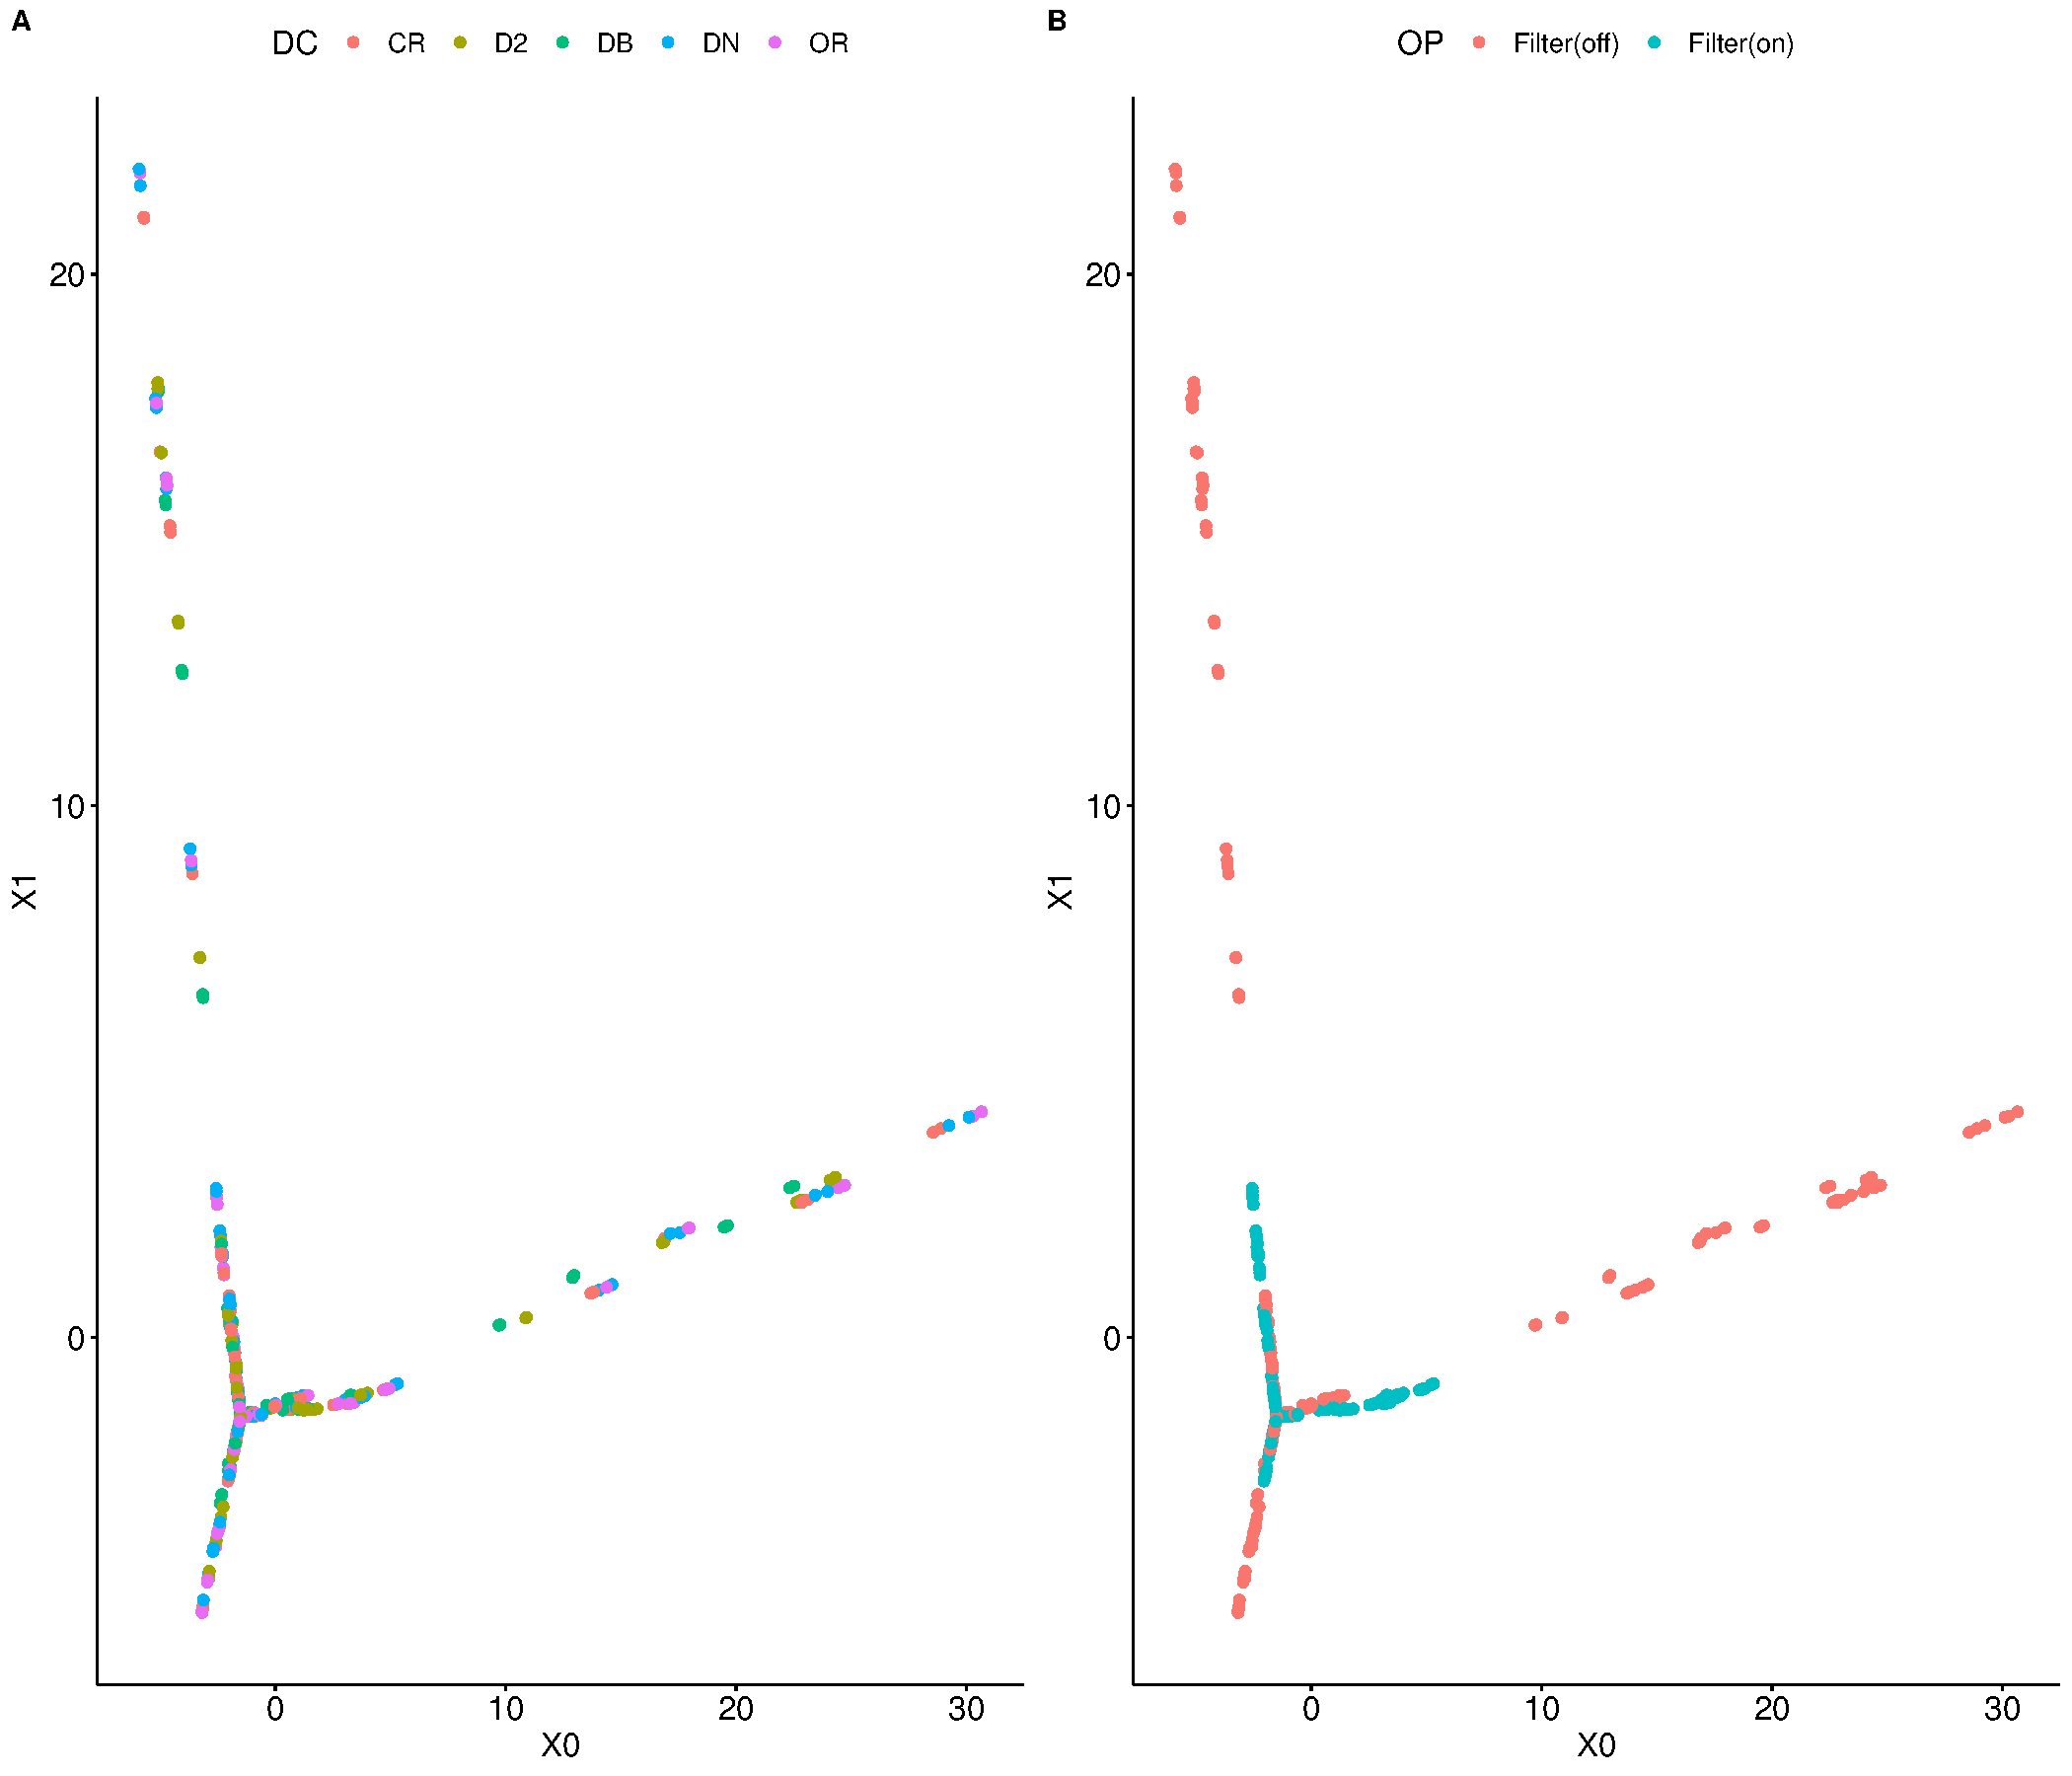
\includegraphics[width=1.0\linewidth]{figure_s1.pdf}
    \end{figure}
    \begin{figure}[H]
      \centering
        \caption{
          \textbf{The networks which were filtered during the \ac{op} step are less variable}
          All combinations of inferred networks are shown as points on a PCA plot and shows the variation in the inferred networks in the first two principal axes (similar to Figure~\ref{fig:figure6}B).
          Each point on the PCA plot represents a network inferred using different combinations of tools and parameters that are available in the \ac{micone} pipeline.
          The points are colored by the tools or parameters used in the \ac{dc} step (A) and the \ac{op} step (B).
          The \ac{dc} step does not seem to have any correlation with the similarity of networks on the PCA plot, but all the networks with filtering at the \ac{op} step are similar to each other.
          This further confirms that the variability in the networks decreases upon filtering out the taxonomic entities at low abundance.
        }
      \label{fig:figure_s1}
    \end{figure}
    \FloatBarrier
    \newpage

    % TODO: Verify this about t-SNE
    \begin{figure}[H]
      \centering
      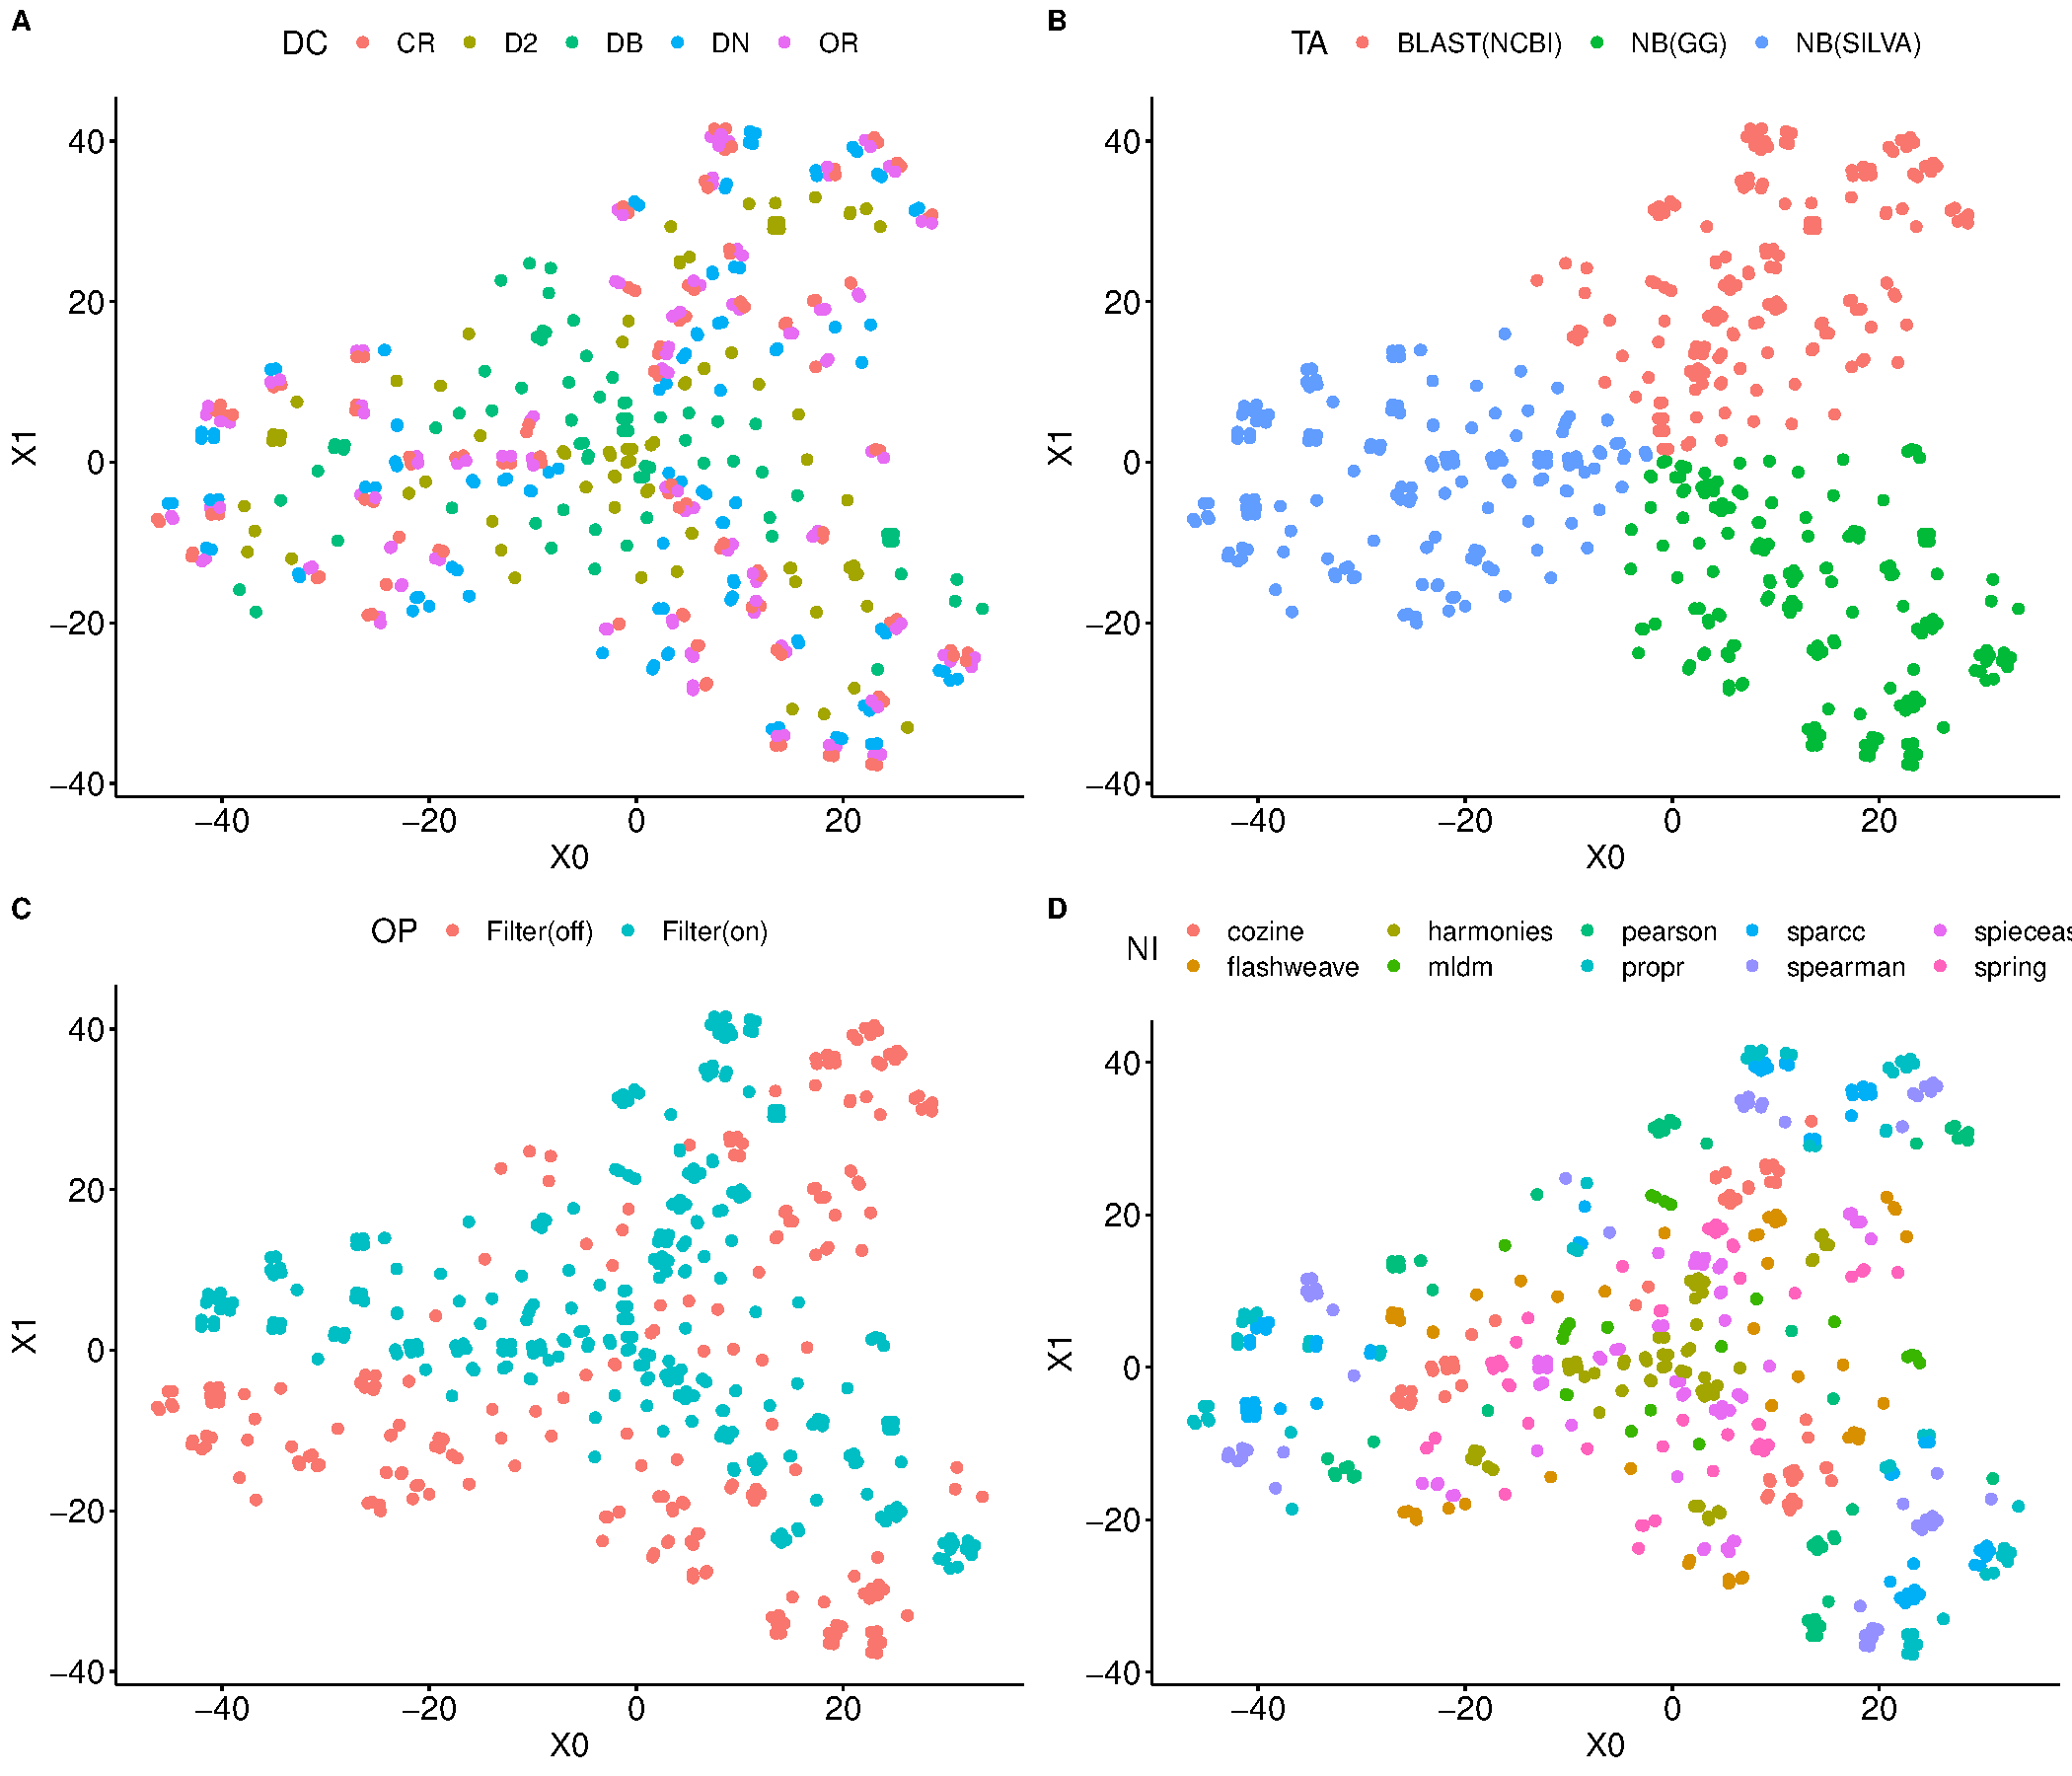
\includegraphics[width=1.0\linewidth]{figure_s2.pdf}
    \end{figure}
    \begin{figure}[H]
      \centering
        \caption{
          \textbf{The t-SNE plot of all the inferred networks clusters the networks based on the taxonomy reference database used}.
          Each point on the t-SNE plot represents a network inferred using different combinations of tools and parameters that are available in the \ac{micone} pipeline.
          The points are colored by the tools and parameters used in \ac{dc} step (A), \ac{ta} step (B), \ac{op} step (C) and \ac{ni} step (D).
          The separation of the points based on taxonomy reference database shows that the points might cluster based on reference database in high-dimensional space.
        }
      \label{fig:figure_s2}
    \end{figure}
    \FloatBarrier
    \newpage

    \begin{figure}[H]
      \centering
      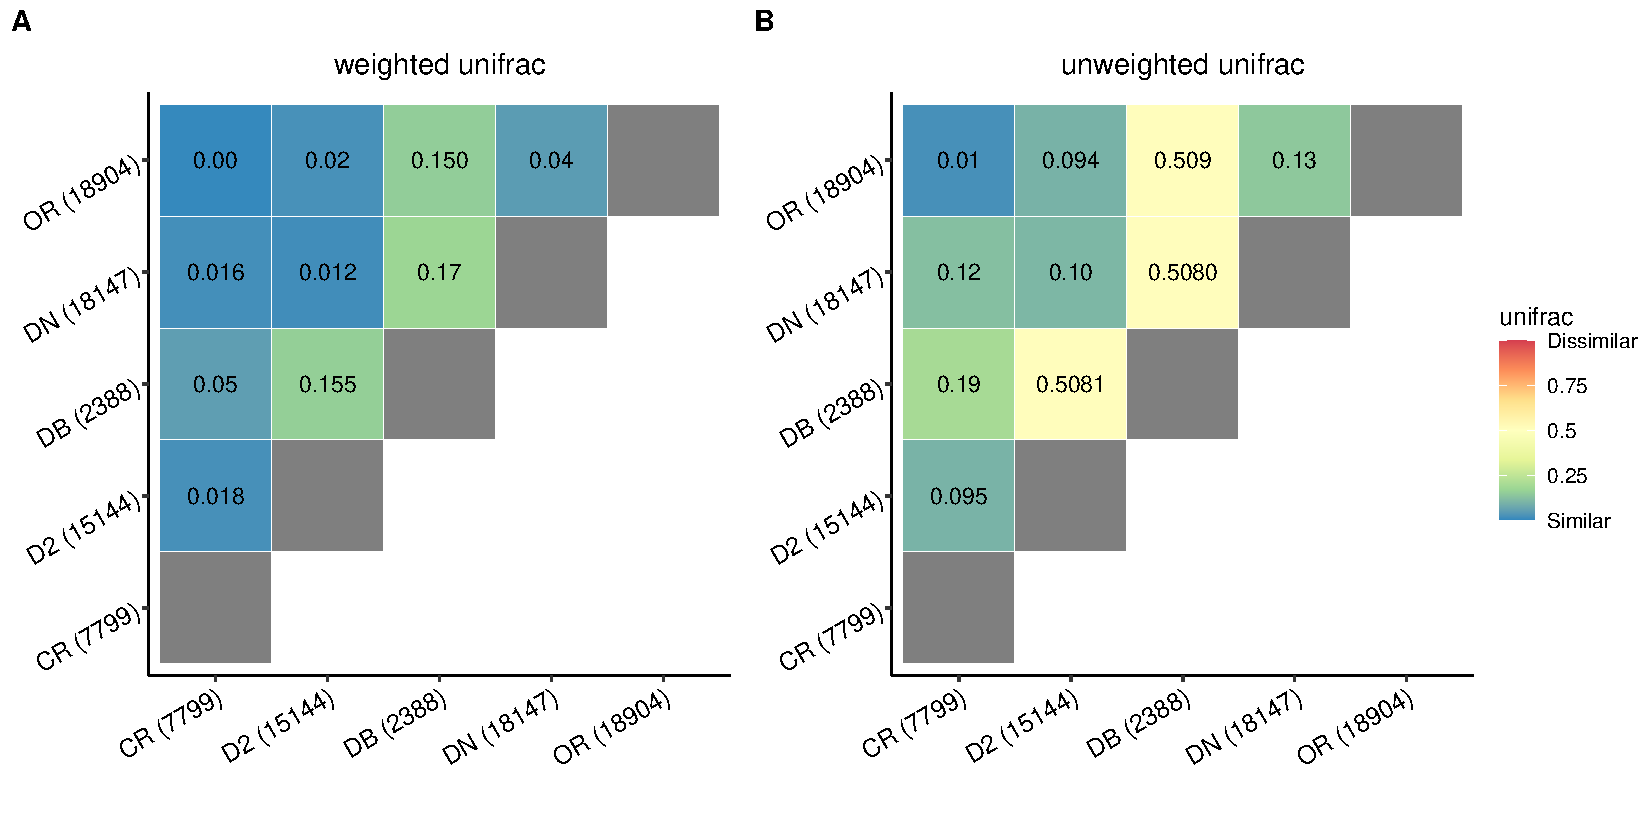
\includegraphics[width=1.0\linewidth]{figure_s3.pdf}
    \end{figure}
    \begin{figure}[H]
      \centering
        \caption{
          \textbf{The UniFrac distance between the 1000 most abundant representative sequences is higher than that when all sequences are considered}.
          Each value is the average UniFrac distance between the reference sequences generated by the various methods in the \ac{dc} step (similar to Figure~\ref{fig:figure2}).
          There is an increase in both weighted and unweighted UniFrac distances compared to when all the representative sequences are considered.
          This shows that the 1000 most abundant representative sequences generated by the methods are not as similar to each other.
          And since the weighted UniFrac is much smaller than the unweighted UniFrac distance, we can conclude that those reference sequences that are present in the middle of the abundance distribution are dissimilar.
        }
      \label{fig:figure_s3}
    \end{figure}
    \FloatBarrier
    \newpage

    \begin{figure}[H]
      \centering
      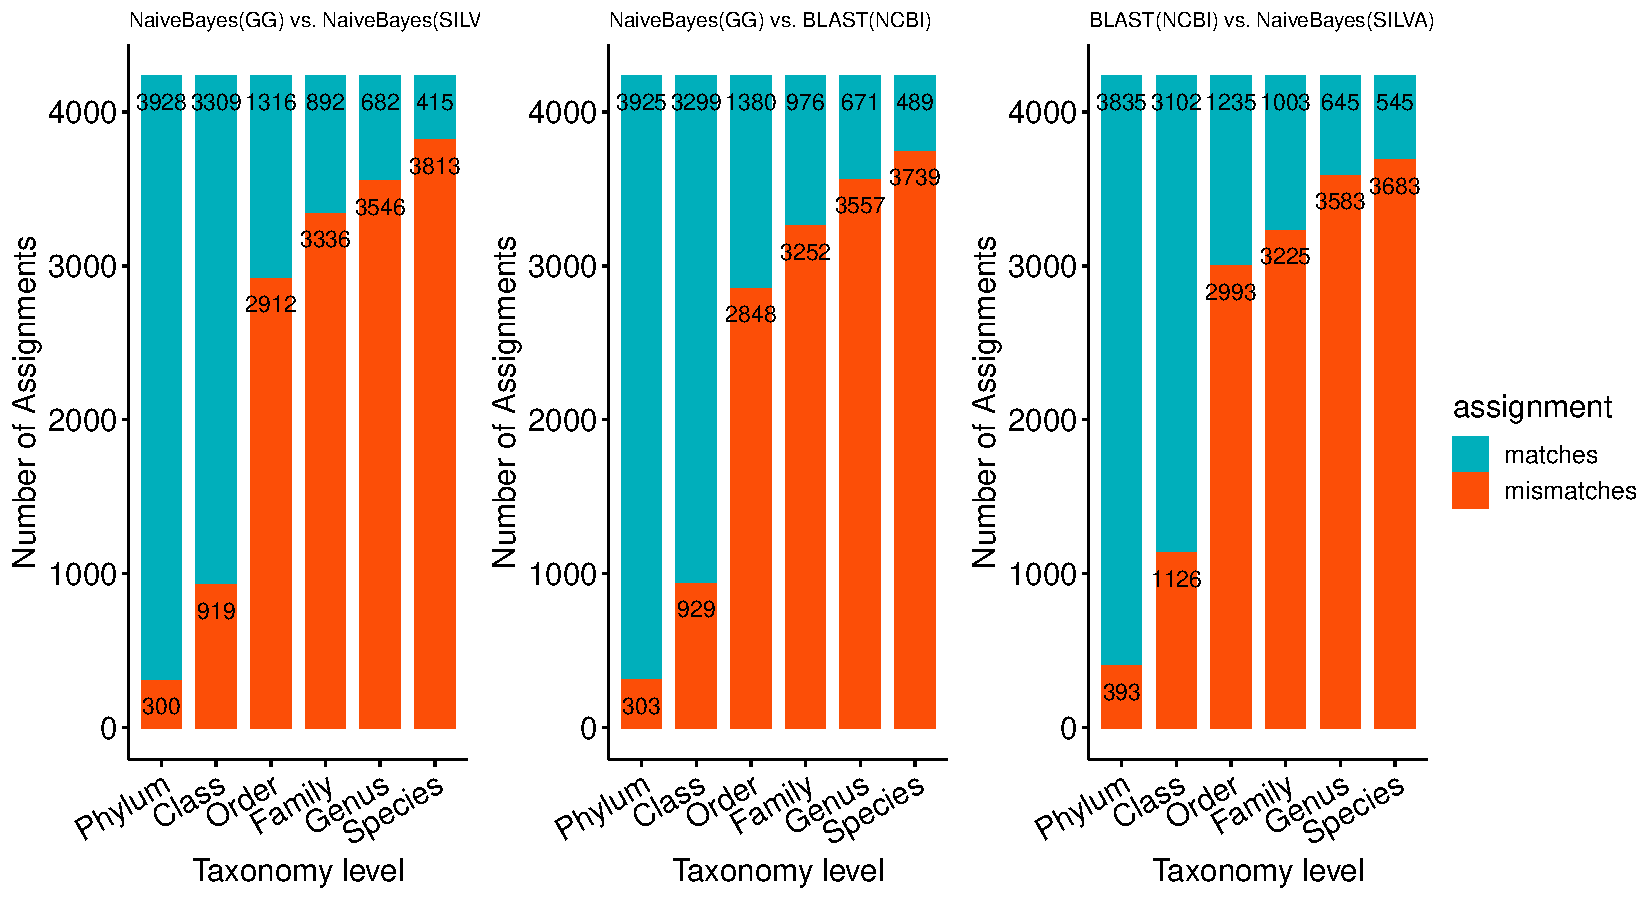
\includegraphics[width=1.0\linewidth]{figure_s4.pdf}
    \end{figure}
    \begin{figure}[H]
      \centering
        \caption{
          \textbf{The weighted and unweighted UniFrac distances between representative sequences generated using remove bimera and uchime for each denoising method are low.}
          The two chimera checking methods, uchime and remove bimera, produce similar outputs.
          With the exception of de novo and open reference under the unweighted UniFrac metric, all the other methods have low dissimilarity.
          This is especially true for the \ac{dada2} and Deblur methods which are the recommended denoising methods in the \ac{micone} pipeline.
          Therefore, remove bimera is recommended as the default chimera method if one is using \ac{dada2} and uchime-denovo when one is using Deblur, since these methods were developed for these respective algorithms (\ac{qiime2} uses uchime-denovo in the Deblur workflow).
        }
      \label{fig:figure_s4}
    \end{figure}
    \FloatBarrier
    \newpage

    \begin{figure}[H]
      \centering
      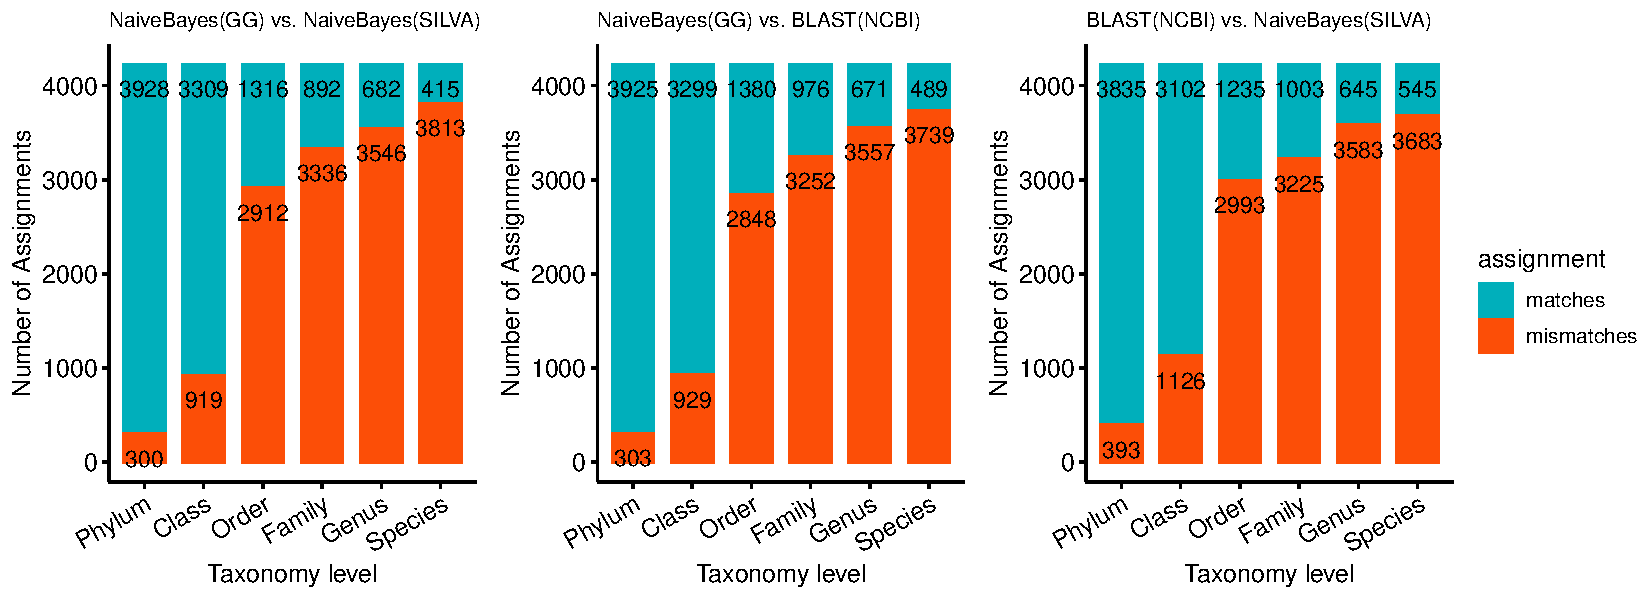
\includegraphics[width=1.0\linewidth]{figure_s5.pdf}
    \end{figure}
    \begin{figure}[H]
      \centering
        \caption{
          \textbf{The pairwise comparison of assignments generated using different databases for all representative sequences has a higher proportion of mismatches}.
          The comparison made here is similar to Figure~\ref{fig:figure3}B, but instead of the top 100 taxonomic entities (by abundance), all the assignments from one database are matched with those from the other two databases.
          Higher percentage of mismatches implies that the matching of the taxonomies in the more abundant sequences (top 100) are more consistent.
        }
      \label{fig:figure_s5}
    \end{figure}
    \FloatBarrier
    \newpage

  \begin{figure}[H]
    \centering
    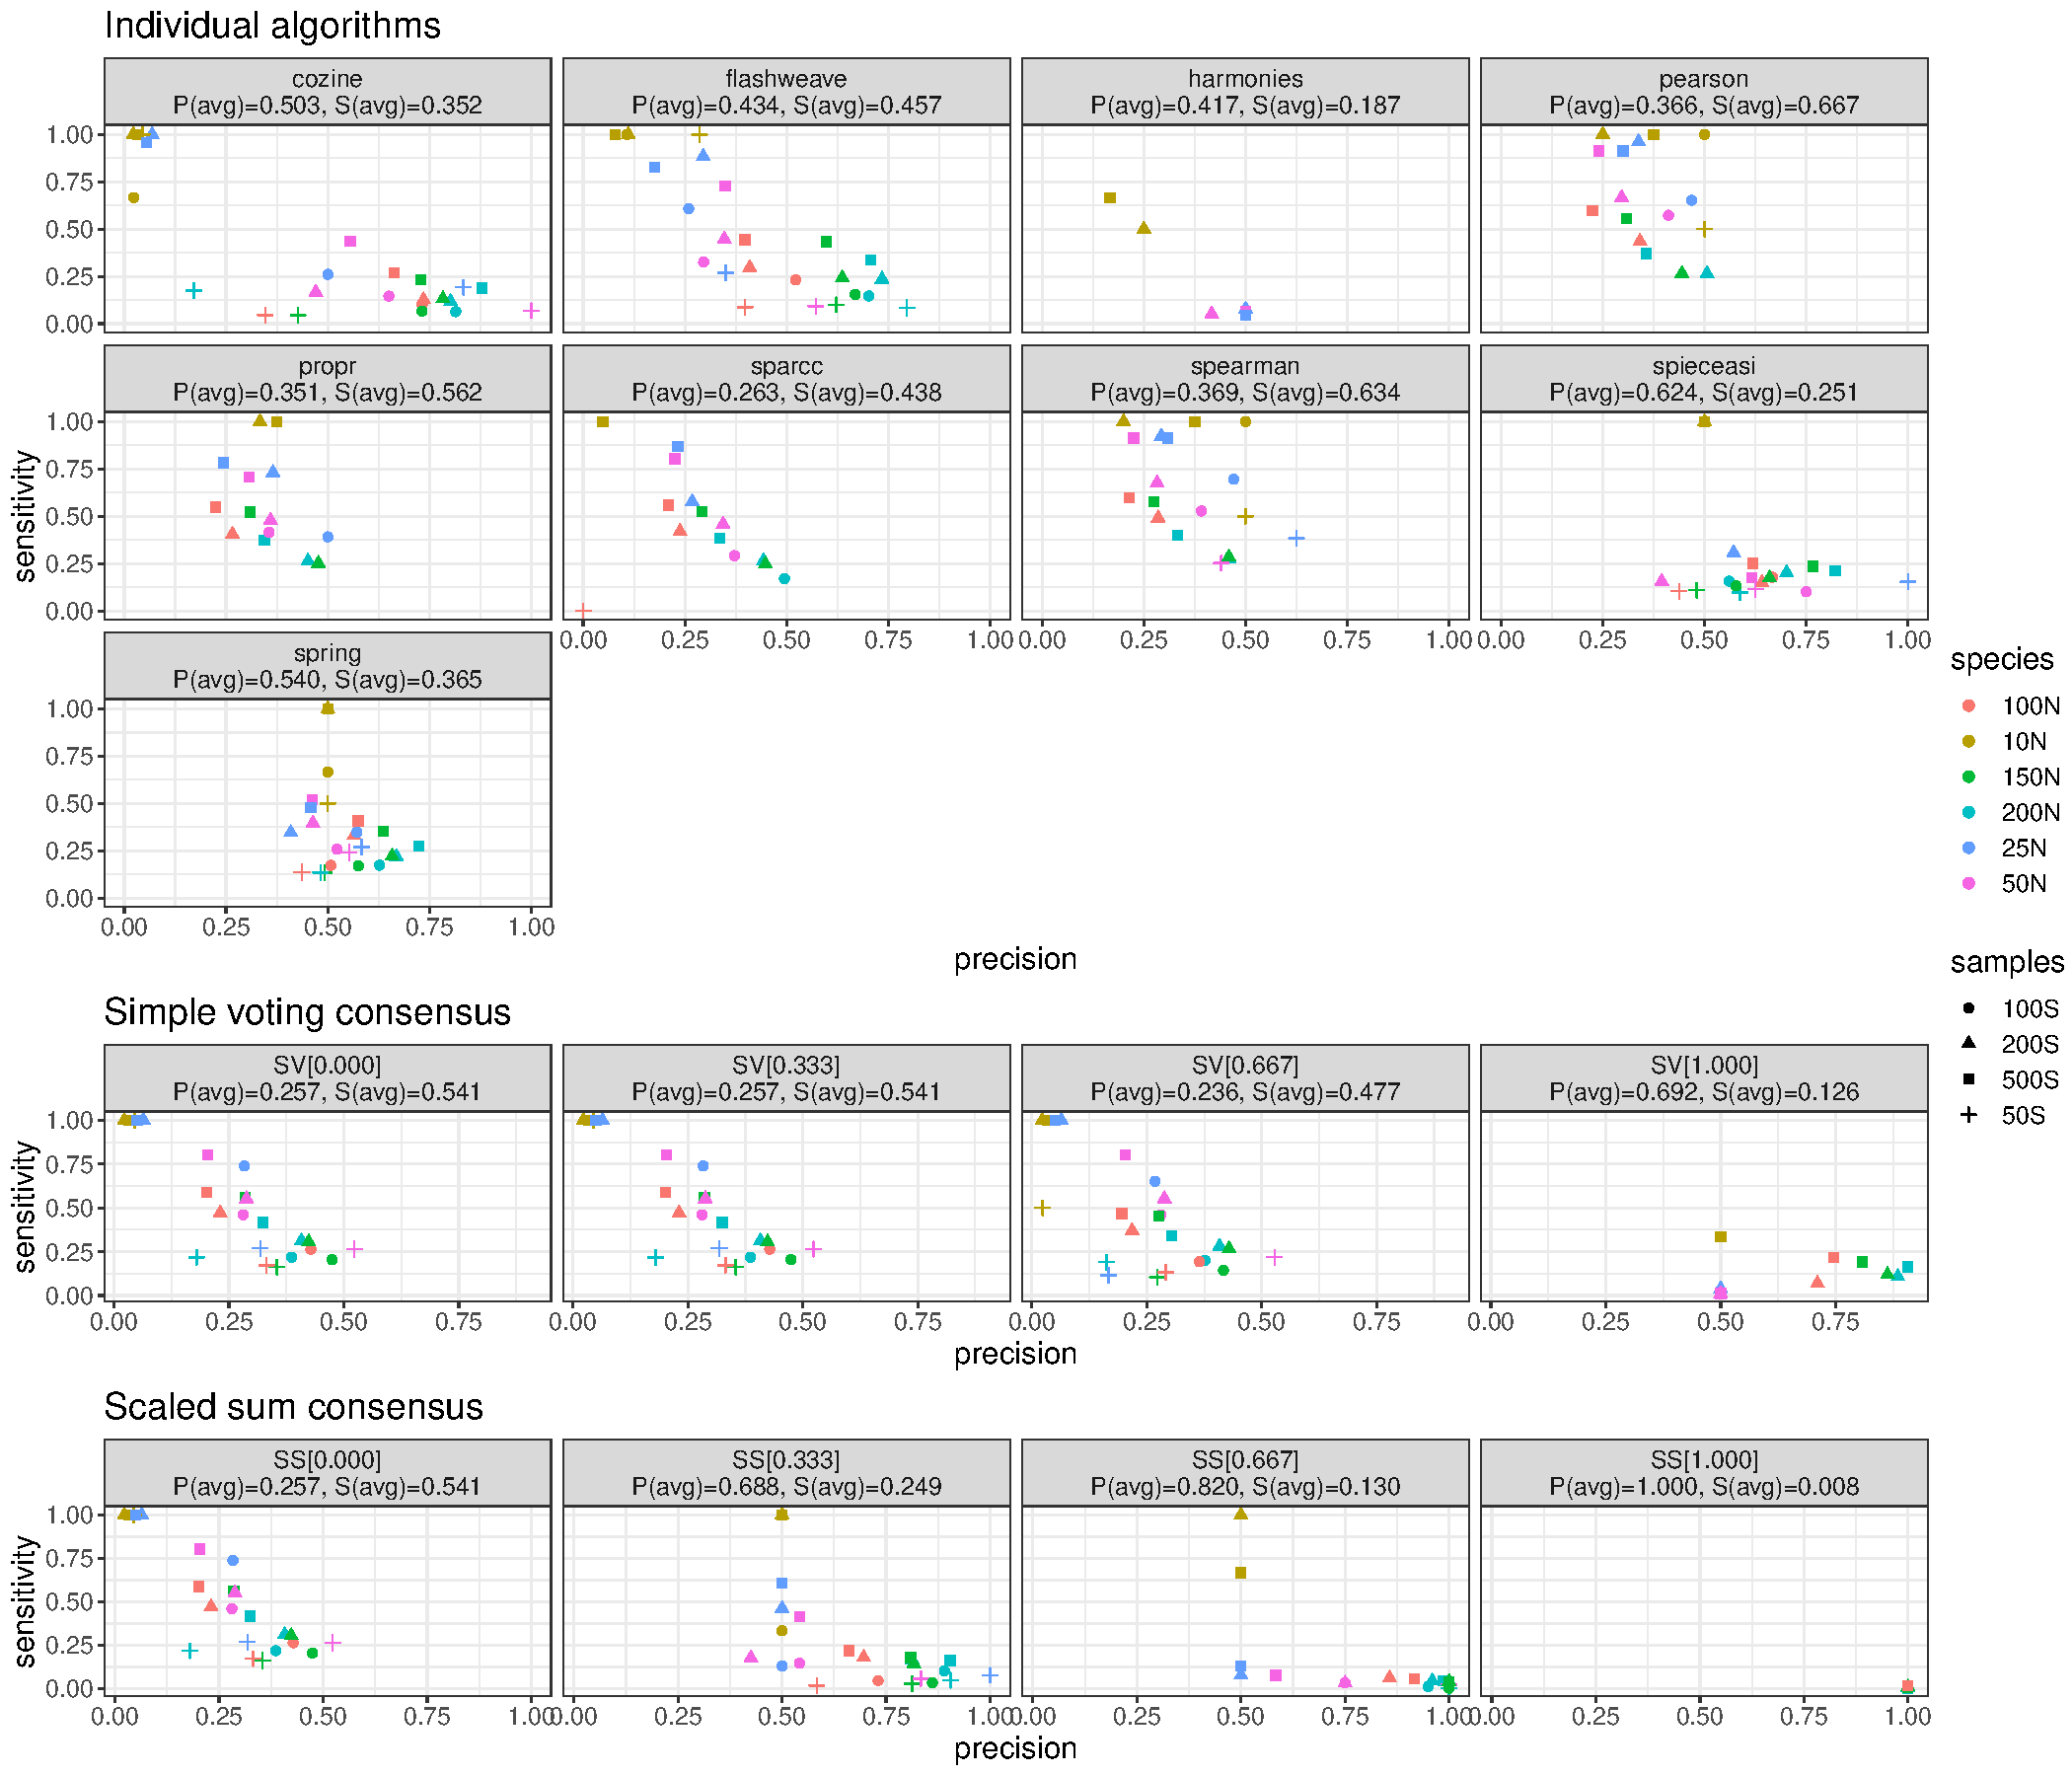
\includegraphics[width=1.0\linewidth]{figure_s6.pdf}
  \end{figure}
  \begin{figure}[H]
    \centering
      \caption{
        \textbf{The precision and sensitivity of the inferred networks on the NorTA synthetic interaction data when Pearson and Spearman are included in the consensus calculation}.
        The ``I'' prefix indicates the individual network inference methods and the ``X'' prefix denotes the different consensus based methods.
        The different consensus based methods used are: pvalue merging (PM), scaled-sum (SS) and simple voting (SV) method.
        With the addition of Pearson and Spearman in the consensus calculation we observe a decrease in the average precision scores of both the consensus algorithms (compared to Figure~\ref{fig:figure5}.
        The overall best precision was still consistently obtained by the scaled-sum method (0.985, 0.963 and 1.000), but the performance was not stable to an increase in the parameter value.
        The simple voting method when using presence of edges in all inferred networks as a requirement (parameter value 1.000), again outperforms \ac{spieceasi} on average precision (0.961).
      }
    \label{fig:figure_s6}
  \end{figure}
  \FloatBarrier
  \newpage

  \begin{figure}[H]
    \centering
    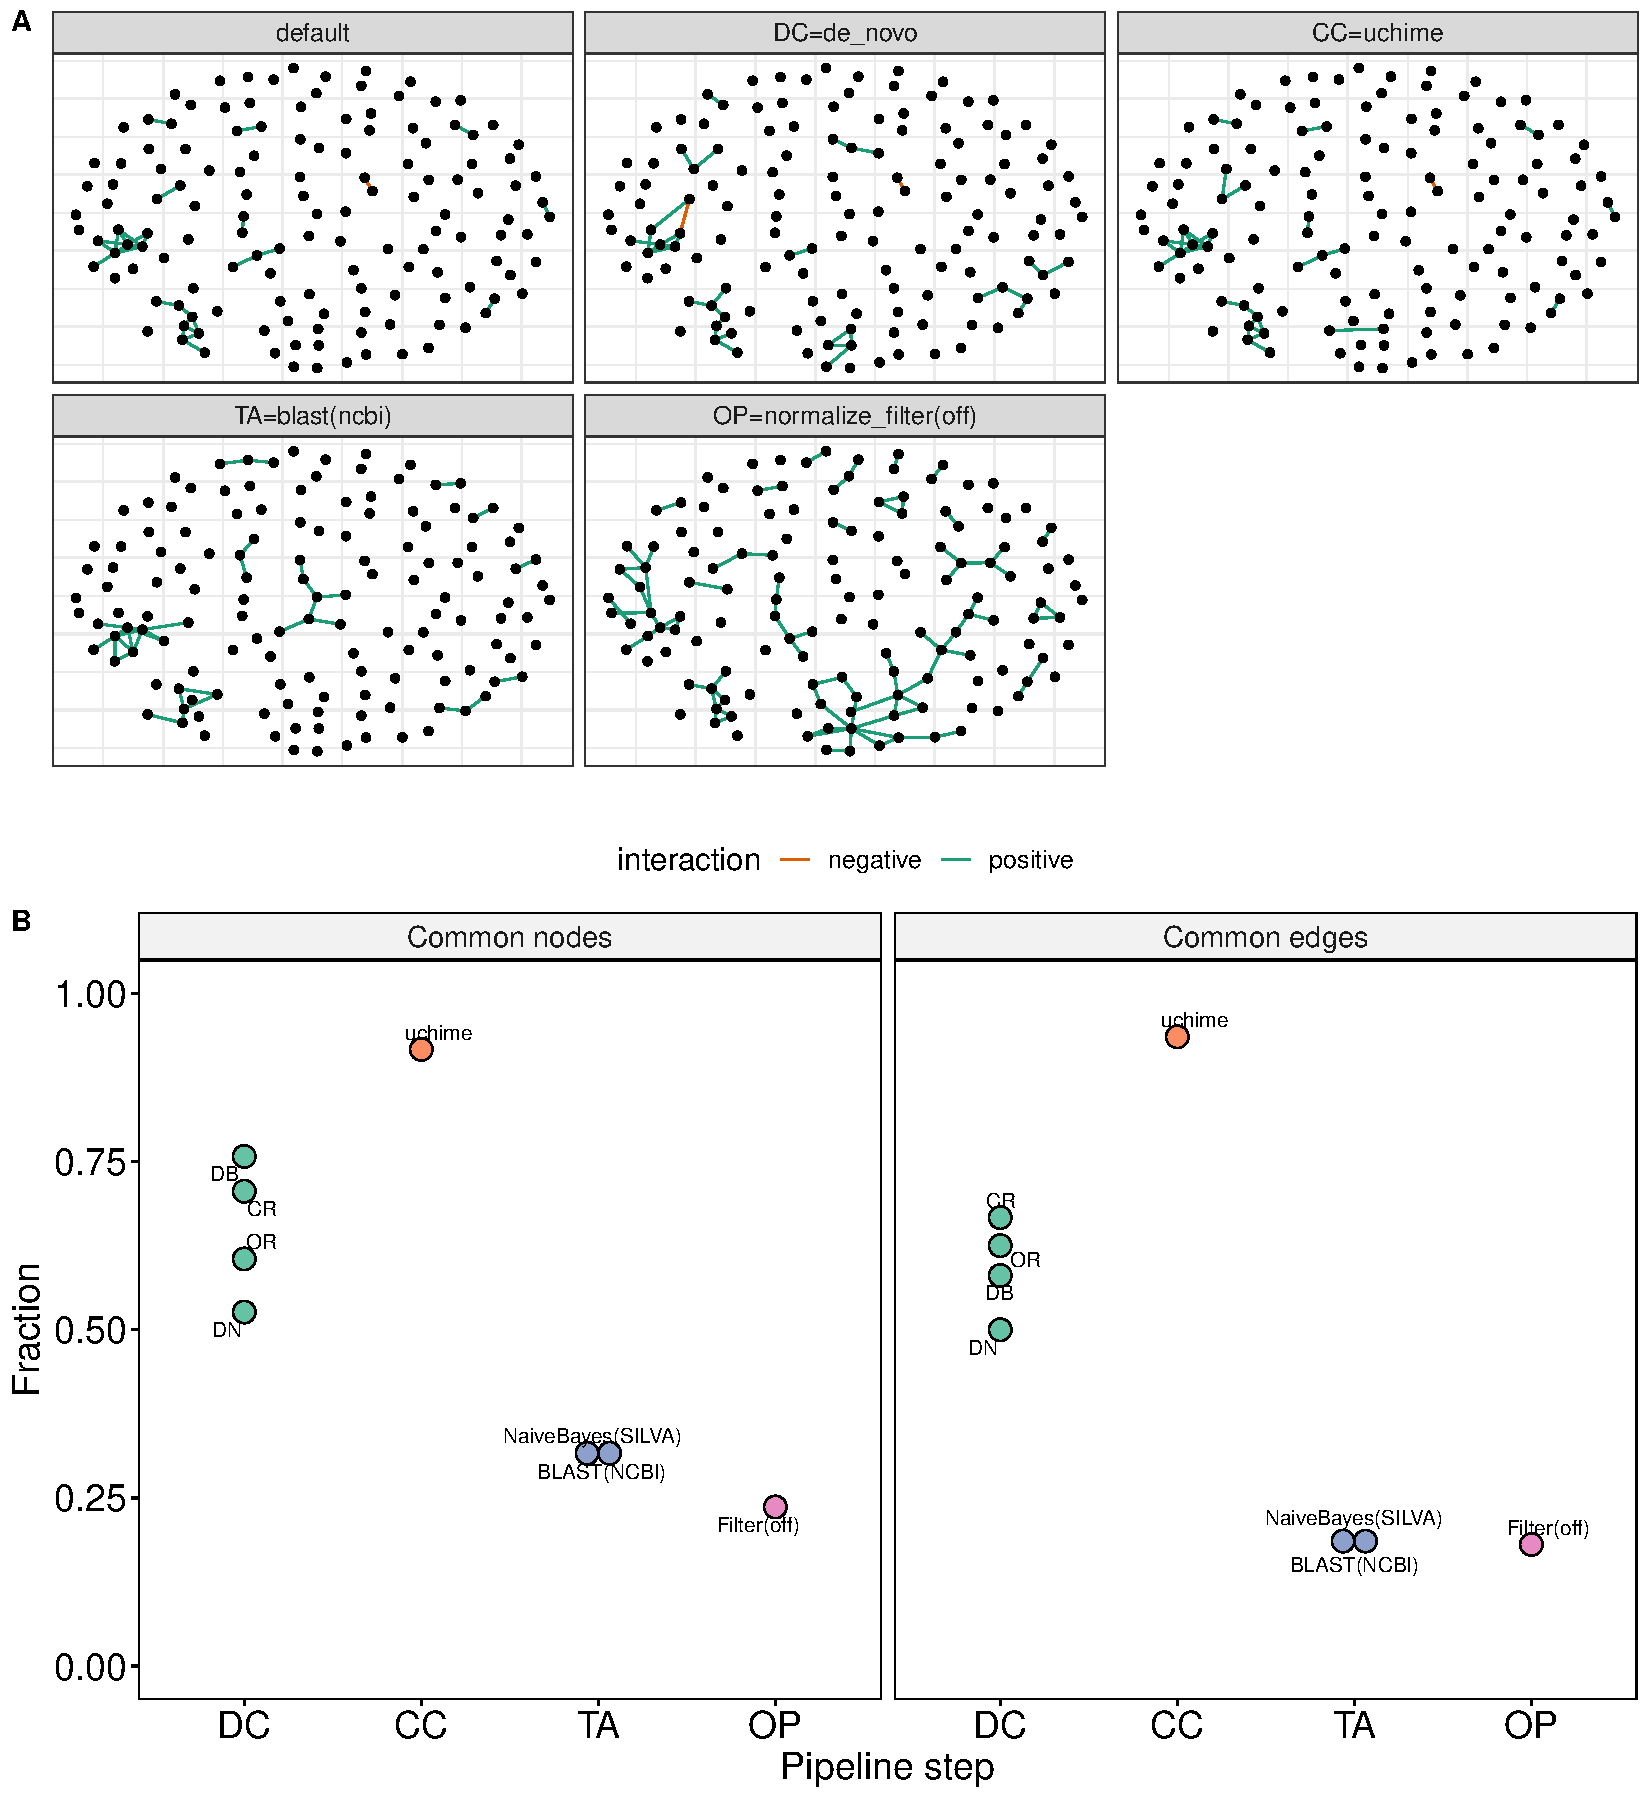
\includegraphics[width=1.0\linewidth]{figure_s7.pdf}
  \end{figure}
  \begin{figure}[H]
    \centering
      \caption{
        \textbf{The precision and sensitivity of the inferred networks on the seqtime synthetic interaction data.}
        The ``I'' prefix indicates the individual network inference methods and the ``X'' prefix denotes the different consensus based methods.
        The different consensus based methods used are: pvalue merging (PM), scaled-sum (SS) and simple voting (SV) method.
        Pearson and Spearman methods are not used in the calculation of the consensus.
        Among all the independent network inference methods, \ac{spieceasi} has the best average precision (0.624), but the overall best precision was consistently obtained by the scaled-sum method (0.688, 0.820 and 1.000).
        The simple voting method when using presence of edges in all inferred networks as a requirement (parameter value 1.000), also outperforms \ac{spieceasi} on average precision (0.692).
        These results show that the scaled-sum method is not only much better suited for inferring robust and accurate interactions from count data regardless of the distributions and topologies.
        But, it is also capable of accurately extracting real interactions (gLV interactions) from count data.
      }
    \label{fig:figure_s7}
  \end{figure}
  \FloatBarrier
  \newpage

  \subsection*{Processing the FMT data}

    \subsubsection*{Data download and pre-processing}
    The main biological dataset used in this study was the collection of 16S rRNA sequencing reads from stool samples (healthy and autistic individuals) for a fecal microbiome transplant study~\cite{Kang2017}.
    The data containing the 16S sequencing reads (V4 region) was downloaded from Qiita~\cite{qiita} (study ID: 10532).
    Only runs 2, 3, and 4 were used for the subsequent analysis as these runs consisted of paired-end sequencing data and run 1 contained single-end data.
    The sample metadata was updated to contain only BMI, sex, height, weight and experimental group.
    This was necessary as two of the network inference algorithms (\ac{mldm} and FlashWeave) required information about environmental heterogeneity.
    However, these environmental correlations were not included in the current analyses.

    \subsubsection*{Processing using the \ac{micone} pipeline}
    The data was then processed using the \ac{micone} pipeline starting at the \ac{sp} step and ending at the \ac{ni} step with the consensus algorithm.
    The configuration files (main.nf and nextflow.config) used to run the \ac{micone} pipeline as well the details of the pipeline execution (dag, report, timeline and trace) are in the "runs/FMT" directory of the data and scripts repository (\href{https://github.com/segrelab/MiCoNE-pipeline-paper}{https://github.com/segrelab/MiCoNE-pipeline-paper})
    % TODO: Store pipeline results
    The results of the pipeline execution for reproducing the analyses in the manuscript are stored on Zenodo[REF] at ...

  \subsection*{Processing the mock data}

    \subsubsection*{Data download and pre-processing}
    The mock datasets, mock4, mock12 and mock16 used for this study, were obtained from mockrobiota~\cite{Bokulich2016}.
    Mock 4 is a mock community composed of 21 bacterial strains represented in equal abundances in two replicate samples, and the same strains represented in uneven abundances in two other replicate samples.
    Mock 12 is composed of 27 bacterial strains containing closely related taxa, the members of which were chosen in part for their well-separated 16S rRNA gene sequences. Some pairs of strains differ by as little as one nucleotide, but all the strains are distinguishable over the sequenced region of the 16S rRNA gene.
    Mock 16 is a mock community composed of even amounts of purified genomic DNA from 49 bacteria and 10 archaea.
    The datasets did not require any preprocessing and could be directly used as input to the pipeline

    \subsubsection*{Processing using the \ac{micone} pipeline}
    The data was processed using the \ac{micone} pipeline starting at the \ac{sp} step and ending at the \ac{op} step with the filtered taxonomic tables as the final output.
    The configuration files (main.nf and nextflow.config) used to run the \ac{micone} pipeline as well the details of the pipeline execution (dag, report, timeline and trace) are in the "runs/mock*" directory of the data and scripts repository (\href{https://github.com/segrelab/MiCoNE-pipeline-paper}{https://github.com/segrelab/MiCoNE-pipeline-paper})
    % TODO: Store pipeline results
    The results of the pipeline execution for reproducing the analyses in the manuscript are stored on Zenodo at ...

% TODO: Update this section and link
    \subsubsection*{Interpretation of Unifrac results in the DC step}
  In order to verify this claim, for each of these methods, we selected the top 1000 representative sequences for each method and recalculated the distance metrics (Figure \ref{fig:figure_s3}).
  We observe that both the weighted and unweighted UniFrac distances are increased, implying that the top representative sequences generated by the different methods are not as similar to each other.
  Therefore, since the weighted UniFrac distances are lower than the unweighted distances, we conclude that the representative sequences in the middle range of the abundance distribution are those that must be the most similar between the methods.
    
    Open-reference and de novo clustering methods perform the best under the weighted UniFrac metric and the worst (marginally) under the unweighted UniFrac metric.
    This result can be attributed to the large number of low abundance representative sequences that are generated by these methods.
    Deblur performs poorly under weighted Unifrac and although its performance on the mock4 dataset is the best under unweighted UniFrac, its performance on the other datasets is average.
    The Deblur method returns a very small number of representative sequences (2388) and this could account for the reason for the high dissimilarity with the other methods as well as irregular performance on the mock data.
    
  \subsection*{Synthetic interaction data}

    \subsubsection*{Data generation}
    The synthetic interaction data for the study were generated using two methods.
    The first method, ``seqtime''~\cite{faustSignaturesEcologicalProcesses2018} utilized generalized Lotka-Volterra (gLV) equations to model the microbial community dynamics and made use of the Klemm–Eguı́luz algorithm to generate clique-based interaction networks~\cite{Rottjers2018}.
    We used the seqtime R package to simulate communities with different numbers of species and samples (see Methods for details).
    The second method, ``NorTA'' used the Normal to Anything (NorTA) approach coupled with a given interaction network topology to generate the abundance distribution of the microbial community~\cite{Kurtz2015}.
    We used the spieceasi R package to simulate communities with different abundance distributions and network topologies (see Methods for details).
    The scripts to generate these datasets can be found in the synthetic data and scripts repository (\href{https://github.com/segrelab/MiCoNE-synthetic-data}{https://github.com/segrelab/MiCoNE-synthetic-data})

    \subsubsection*{Processing using the \ac{micone} pipeline}
    The data was processed using the \ac{micone} pipeline using only the \ac{ni} step with the consensus networks as the final output.
    The configuration files (main.nf and nextflow.config) used to run the \ac{micone} pipeline as well the details of the pipeline execution (dag, report, timeline and trace) are in the "runs/norta" and "runs/seqtime" directories of the data and scripts repository (\href{https://github.com/segrelab/MiCoNE-pipeline-paper}{https://github.com/segrelab/MiCoNE-pipeline-paper})
    % TODO: Store pipeline results
    The results of the pipeline execution for reproducing the analyses in the manuscript are stored on Zenodo at ...


  \subsection*{Network metrics}

  In Table~\ref{tab:network_metrics} we show various global network metrics calculated for each tool in the pipeline.
  All the networks that make use of a particular tool are grouped together, and the following average metrics are calculated for each group:
  \begin{enumerate}
    \item The average shortest path length describes the average of all the shortest paths in the graph. No number is reported if the graph is not connected, therefore, the results indicate that none of the networks that make use of \ac{harmonies}, \ac{cozine}, \ac{spring}, \ac{spieceasi} and Pearson are connected.
    \item The average clustering is the average clustering coefficient of the graph. The closer the value is to 1.0, the more densely connected is the graph. We can observe that the networks that use correlation-based methods have the highest values while the direct-association based methods have the lowest.
    \item The number of connected components is the highest for the direct-association based methods and the lowest for the correlation-based methods. In the case of propr, all the networks have only one giant component.
    \item The modularity metric is the modularity over all partitions in a graph calculated using a label propagation algorithm~\cite{cordascoCommunityDetectionSemisynchronous2010}. Positive values imply that there are more edges between vertices of the same type than we would expect by chance, and negative implies that there are less. The networks inferred by \ac{mldm} report very few edges, and skew the average modularity scores. This could also be an artifact of incomplete converge of the \ac{mldm} algorithm for some combinations.
    \item Node connectivity refers to the minimum number of nodes that must be removed from the graph to make it disconnected. We observe that only the networks generated using propr have a high value since most of these networks are connected.
    \item Degree assortativity coefficient measures the similarity of connections in the graph with respect to the node degree. Again we observe that the direct-association based methods have negative degree assortativity, meaning that there are many hubs in these networks. The correlation-based methods have positive values implying that in these networks nodes with similar degrees attach to one another.
  \end{enumerate}
  All the metrics were calculated using the \texttt{networkx} Python package~\cite{hagbergExploringNetworkStructure2008}.

  \subsection*{p-value merging}

  Fisher~\cite{fisher_224a_1948} proposed that for $k$ independent p-values, each generated by $k$ different methods and denoted by $\bar{P}^i$ (notations are same as used in the "Consensus network and p-value merging" subsection of the Methods), the following will hold true for the statistic $\Psi$:
  \begin{equation*}
    \begin{aligned}
      \Psi &= \sum_{i=1}^k -2 \log \left( \bar{P}^i \right) \\
        \Psi &\sim \chi^2_{2k}
    \end{aligned}
  \end{equation*}

  Brown~\cite{brown_400_1975} extended Fisher's method to dependent p-values by using a re-scaled $\chi^2$ distribution:
  \begin{equation*}
    \Psi \sim c \chi^2_{2f}
  \end{equation*}
  where, $f$ is the degrees of freedom and $c$ is the scale factor and are given by:
  \begin{equation*}
    f = \frac{\mathrm{E}[\Psi]^2}{\mathrm{Var}[\Psi]} ~~~\text{and}~~~ c = \frac{\mathrm{Var}[\Psi]}{2\mathrm{E}[\Psi]} = \frac{k}{f}
  \end{equation*}

  Furthermore, Brown showed that $\mathrm{E}[\Psi]$ and $\mathrm{Var}[\Psi]$ can be calculated via a numerical integration:
  \begin{equation*}
    \mathrm{E}[\Psi] = 2k ~~~\text{and}~~~ \mathrm{Var}[\Psi] = 4k + 2\sum_{i<j} \mathrm{Cov}\left( -2\log(\bar{P}^i), -2\log(\bar{P}^j) \right)
  \end{equation*}

  Kost and McDermott~\cite{kost_combining_2002} further fit a third-order polynomial to approximate the covariance
  \begin{equation}
    \mathrm{Cov}\left( -2\log(\bar{P}^i), -2\log(\bar{P}^j) \right) \approx 3.263 \rho_{ij} + 0.710 \rho_{ij}^2 + 0.027 \rho_{ij}^3
    \label{eqn:suppl_covariance-pvalues}
  \end{equation}
  where, $\rho_{ij}$ is the correlation between method $i$ and method $j$

  The final combined p-value~\cite{Poole_Gibbs_Shmulevich_Bernard_Knijnenburg_2016} is then given by:
  \begin{equation}
    \begin{aligned*}
        & \hat{P}_j = 1.0 - \Phi_{2f}\left( \psi / c \right) \\
        \text{where},~ &\psi = -2 \sum_{i=1}^k \log(\bar{P}^i_j) ~~~\text{and}~~~ \Phi_{2f} = \mathrm{CDF}\left( \chi^2_{2f} \right)
    \end{aligned*}
    \label{eqn:suppl_pvalue-combined}
  \end{equation}

  The p-value merging and consensus method in \ac{micone} (refer Methods) uses Equation~\ref{eqn:suppl_covariance-pvalues} to estimate the covariance of the p-values and Equation~\ref{eqn:suppl_pvalue-combined} to merge the p-values (obtained from bootstrapping) from the different correlation methods.
  Note that we do not use Pearson and Spearman methods in the p-value merging step and these algorithms are only used for demonstration and comparison.
  The combined p-values are used to threshold for significance the correlation-based networks during the consensus network step.

  % TODO: Should we mention the MIND database here?
  \subsection*{The JSON network format and network exports}

    The default format \ac{micone} uses for storing the network files is the JSON (JavaScript Object Notation) format.
    The custom JSON schema we have designed is able to store all network related information pertaining to nodes, links and the metadata related to the links and datasets.
    Additionally, \ac{micone} also supports exporting of networks into a variety of other formats such as edge lists, .gml and cytoscape formats.
    Since, we make use of \texttt{networkx}~\cite{hagbergExploringNetworkStructure2008} for the export functionality, networks can be exported to all formats supported by the package.
    However, not all the corresponding metadata will be exported appropriately, since most formats do not support this additional metadata.
    The details of the format and information about importing/exporting it and other network formats can be found in the \ac{micone} documentation.

  \subsection*{Supplementary discussion}

  Additionally, it is worth pointing out some additional more specific conclusions stemming from the individual steps of our analysis.
  The different denoising/clustering methods differ mostly in their identification of sequences that are in low abundances.
  Hence, they do not have much of an impact on the inferred co-occurrence networks when the sequences of low abundance are removed (Figure~\ref{fig:figure_s1}).
  Comparison of inferred and expected reference sequences and their abundances in mock community datasets has allowed us to identify \ac{dada2} as the method which best recapitulates the expected sequence composition.
  For the chimera checking module, we suggest using the remove bimera method since it was developed in conjunction with \ac{dada2} and its performance does not significantly differ from uchime-denovo.
  For the current work we have decided to focus on the tools most widely used at the time of the analysis.
  Some tools which were not as widely used (e.g. dbOTU3~\cite{Olesen2017}) as well as older popular methods like mothur~\cite{Schloss2009} have not been included in the study, but could be added into the pipelines in future updated analyses.

  The choice of taxonomy database was found to be the most important factor in the inference of microbial co-occurrence networks, contributing $65.4\%$ of the total variance.
  The frequent changes in the taxonomy nomenclature coupled with the frequency of updates to the various 16S reference databases create inherent differences \cite{Balvociute2017} in taxonomy hierarchies in these databases.
  Our analysis revealed that no particular reference database performs better than the others across the different mock dataset benchmarks.
  The default reference database in the pipeline is the \ac{gg} reference database along with the ``Naive Bayes'' classifier as the query tool.
  The reason for our choice stems from the popularity of the \ac{gg} database~\cite{parkEvaluation16SRRNA2018} in taxonomic studies, which would enable easy comparison across datasets.
  However, for newer studies we recommend using SILVA database because of its size and taxonomic comprehensiveness~\cite{iiRESCRIPtReproducibleSequence2021} and since \ac{gg} has not been updated since 2013.
  Additionally, a particular database might be more appropriate than the rest based on specific requirements.
  For example, in order to generate a dataset that is compatible with the \ac{mind} platform~\cite{huResourceComparisonIntegration2022} \ac{ncbi} is the most appropriate choice as it guarantees compatibility of taxonomic hierarchy and therefore comparability with other datasets.
  Furthermore, we also enable users to use custom databases~\cite{Ritari2015,iiRESCRIPtReproducibleSequence2021} with the BLAST and Naive Bayes classifiers that are incorporated into the pipeline (from \ac{qiime2}).
  We suggest that that choice of the database should be made based on possible reported or inferred biases in the representation of given biomes in a specific databases~\cite{Balvociute2017,iiRESCRIPtReproducibleSequence2021}, as choosing taxon-specific databases have also been observed to compromise classification~\cite{rmarcelinoUseTaxonspecificReference2020}.

  The \ac{op} step of the pipeline is second in its contribution to total network variance.
  This can be attributed to the large number of nodes that are added to the final networks when the filtering is turned off.
  Additionally, a very large number of nodes also decreases the accuracy of the network inference algorithms for the same sample size~\cite{peschelNetCoMiNetworkConstruction2020} and increases the computational complexity~\cite{tackmannRapidInferenceDirect2019}.
  We observe that filtering out taxa that are present in low abundances in all samples increases the proportion of taxa in common between taxonomy tables generated using different reference databases (Figure~\ref{fig:figure_s5}), providing another reason for filtering.
  We also observe that the reduction in the number of taxa leads to better agreement in the networks inferred through different methods (Figure~\ref{fig:figure_s1}).
  Moreover, filtering is necessary in order to increase the power in tests of significance when the number of taxa is much greater than the number of samples.
